% Figure clh_lean_inverse: level sets of F_y = Psi_f - <y, .> on a plane of the slice, its minimizer and damped Newton iterates.
% Illustrates CLH-1 (Section sec:homeo: variational inverse). Inputs: f-bar = (3,5,1,2,4), theta/pi = (0, 0.1, 0.7, 0.3, 0.8), y = G_f(theta); the plane is theta + pi (s e_3 + t e_2).
% Source of the figure, typeset in the paper's own fonts (T1, Latin Modern, 11pt) at the paper's text
% width (6.5in), so \includegraphics does not rescale it. It adds no assertion.
% Every coordinate is read from numerical values computed by floating-point code that follows the
% paper's formulas (the pictures' Lean helper); the SHA-256 of each output line it comes from:
%   D60_s59_default fe00e5317047658c8be31cfb255bdbf9926745fbd095d5002fea9f00f845b572
% Build: pdflatex <this file> && pdftocairo -svg <this file>.pdf <this file>.svg

\documentclass[11pt]{standalone}
\usepackage[T1]{fontenc}
\usepackage{lmodern}
\usepackage{amsmath,amssymb}
\usepackage{tikz}
\usetikzlibrary{arrows.meta,calc}

% the palette of the paper's other figures: blue solid for the first object, ochre dashed for the second
\definecolor{ink}{HTML}{233740}
\definecolor{muted}{HTML}{65757D}
\definecolor{pblue}{HTML}{0072B2}
\definecolor{qochre}{HTML}{B87827}

\tikzset{
  ax/.style={draw=muted, line width=0.5pt},
  axd/.style={draw=muted!70, line width=0.4pt, dash pattern=on 1.5pt off 2pt},
  tick/.style={draw=muted, line width=0.5pt},
  lab/.style={font=\footnotesize, inner sep=1.2pt, text=ink},
  labm/.style={font=\small, inner sep=1.2pt, text=ink},
  labw/.style={font=\footnotesize, inner sep=1pt, text=ink, fill=white, fill opacity=0.8, text opacity=1},
  labP/.style={font=\footnotesize, inner sep=1.2pt, text=pblue},
  labQ/.style={font=\footnotesize, inner sep=1.2pt, text=qochre},
  tk/.style={font=\footnotesize, inner sep=1pt, text=muted},
  panel/.style={font=\small, inner sep=0pt, text=ink},
  curveP/.style={pblue, line width=1.1pt, line cap=round, line join=round},
  thinP/.style={pblue, line width=0.8pt, line cap=round, line join=round},
  thinQ/.style={qochre, line width=0.8pt, dash pattern=on 3pt off 1.6pt, line cap=round, line join=round},
  curveQ/.style={qochre, line width=1.1pt, dash pattern=on 4pt off 1.6pt, line cap=round},
  fillP/.style={pblue, fill=pblue!8, line width=1.1pt, line join=round},
  dotI/.style={circle, draw=ink, fill=ink, line width=0.6pt, inner sep=0pt, minimum size=4.6pt},
  dotIs/.style={circle, draw=ink, fill=ink, line width=0.5pt, inner sep=0pt, minimum size=3.2pt},
  ringI/.style={circle, draw=ink, fill=white, line width=0.6pt, inner sep=0pt, minimum size=4.6pt},
  dotP/.style={circle, draw=pblue, fill=pblue, line width=0.6pt, inner sep=0pt, minimum size=4.6pt},
  dotQ/.style={circle, draw=qochre, fill=qochre, line width=0.6pt, inner sep=0pt, minimum size=4.6pt},
  dotQs/.style={circle, draw=qochre, fill=qochre, line width=0.5pt, inner sep=0pt, minimum size=3pt},
  ringQ/.style={circle, draw=qochre, fill=white, line width=0.6pt, inner sep=0pt, minimum size=4.6pt},
}

\begin{document}
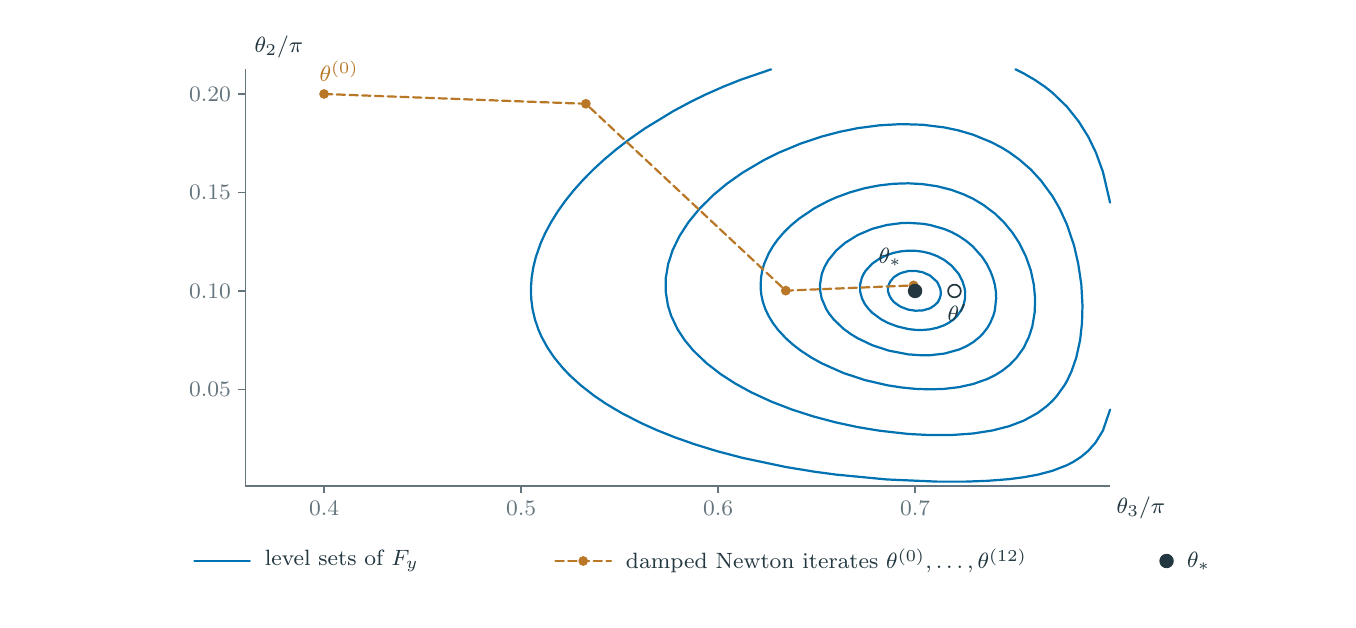
\begin{tikzpicture}[x=1bp,y=1bp]
\useasboundingbox (0bp,0bp) rectangle (468bp,206bp);
%box A 78.32803315 41 311.3439337 150 0.36 0.799 0.001 0.2125024347
\draw[ax] (78.33,41.00) -- (389.67,41.00); %line
\draw[ax] (78.33,41.00) -- (78.33,191.00); %line
\draw[tick] (106.70,41.00) -- (106.70,38.50); %tickx A 0.4
\node[tk] at (106.70,33.00) {$0.4$}; %num A-xt 0.4
\draw[tick] (177.62,41.00) -- (177.62,38.50); %tickx A 0.5
\node[tk] at (177.62,33.00) {$0.5$}; %num A-xt 0.5
\draw[tick] (248.54,41.00) -- (248.54,38.50); %tickx A 0.6
\node[tk] at (248.54,33.00) {$0.6$}; %num A-xt 0.6
\draw[tick] (319.46,41.00) -- (319.46,38.50); %tickx A 0.7
\node[tk] at (319.46,33.00) {$0.7$}; %num A-xt 0.7
\draw[tick] (78.33,75.75) -- (75.83,75.75); %ticky A 0.05
\node[tk, anchor=east] at (74.33,75.75) {$0.05$}; %num A-yt 0.05
\draw[tick] (78.33,111.21) -- (75.83,111.21); %ticky A 0.1
\node[tk, anchor=east] at (74.33,111.21) {$0.10$}; %num A-yt 0.1
\draw[tick] (78.33,146.67) -- (75.83,146.67); %ticky A 0.15
\node[tk, anchor=east] at (74.33,146.67) {$0.15$}; %num A-yt 0.15
\draw[tick] (78.33,182.13) -- (75.83,182.13); %ticky A 0.2
\node[tk, anchor=east] at (74.33,182.13) {$0.20$}; %num A-yt 0.2
\node[lab, anchor=west] at (390.67,33.00) {$\theta_3/\pi$}; %t A-x
\node[lab, anchor=west] at (80.33,199.00) {$\theta_2/\pi$}; %t A-y
\draw[thinP] (317.03,104.49) -- (314.43,105.46) -- (313.53,106.00) -- (311.84,107.22) -- (310.82,108.50) -- (310.13,109.75) -- (309.75,111.00) -- (309.70,112.25) -- (309.99,113.50) -- (310.63,114.75) -- (311.84,116.19) -- (313.52,117.25) -- (314.43,117.70) -- (317.03,118.38) -- (319.62,118.45) -- (322.21,117.95) -- (324.81,116.80) -- (327.40,114.49) -- (328.48,112.25) -- (328.71,111.00) -- (328.67,109.75) -- (328.34,108.50) -- (327.71,107.25) -- (326.44,106.00) -- (324.81,104.95) -- (322.21,104.22) -- (319.62,104.10) -- (317.03,104.49); %poly A/c0-0
\draw[thinP] (319.62,97.21) -- (317.03,97.50) -- (312.88,98.50) -- (309.61,99.75) -- (307.27,101.00) -- (304.05,103.36) -- (302.72,104.75) -- (301.46,106.37) -- (300.36,108.50) -- (299.69,111.00) -- (299.67,113.50) -- (300.31,116.00) -- (300.89,117.25) -- (301.67,118.50) -- (304.05,121.06) -- (306.65,122.85) -- (309.24,124.10) -- (311.84,124.96) -- (314.43,125.48) -- (317.03,125.73) -- (319.62,125.68) -- (322.21,125.36) -- (324.81,124.74) -- (327.40,123.76) -- (330.00,122.36) -- (332.59,120.35) -- (335.19,117.33) -- (336.51,114.75) -- (337.29,112.25) -- (337.49,111.00) -- (337.47,108.50) -- (336.87,106.00) -- (336.33,104.75) -- (334.66,102.25) -- (333.35,101.00) -- (331.59,99.75) -- (330.00,98.89) -- (327.40,97.95) -- (324.81,97.40) -- (322.21,97.17) -- (319.62,97.21); %poly A/c1-0
\draw[thinP] (317.03,88.38) -- (309.94,89.75) -- (304.05,91.69) -- (298.86,94.16) -- (296.27,95.73) -- (293.67,97.63) -- (290.14,101.00) -- (288.49,103.10) -- (287.46,104.75) -- (285.85,108.50) -- (285.35,111.00) -- (285.24,113.50) -- (285.89,117.39) -- (286.81,119.75) -- (288.20,122.25) -- (291.08,125.77) -- (294.24,128.50) -- (298.86,131.38) -- (304.05,133.58) -- (309.24,134.96) -- (314.43,135.64) -- (317.03,135.74) -- (322.21,135.41) -- (324.81,134.98) -- (330.00,133.50) -- (332.59,132.41) -- (335.19,131.03) -- (337.78,129.30) -- (340.24,127.25) -- (343.58,123.50) -- (345.25,121.00) -- (346.51,118.50) -- (347.48,116.00) -- (348.18,113.50) -- (348.55,111.00) -- (348.66,108.50) -- (348.16,104.12) -- (347.61,102.25) -- (346.54,99.75) -- (345.56,98.02) -- (343.99,96.00) -- (342.82,94.75) -- (340.38,92.77) -- (337.78,91.23) -- (335.19,90.10) -- (330.00,88.67) -- (324.81,88.08) -- (322.21,88.04) -- (317.03,88.38); %poly A/c2-0
\draw[thinP] (319.62,75.97) -- (314.43,76.49) -- (309.56,77.25) -- (301.46,79.12) -- (293.67,81.68) -- (285.89,85.15) -- (282.11,87.25) -- (278.29,89.75) -- (275.51,91.89) -- (272.92,94.21) -- (270.10,97.25) -- (268.23,99.75) -- (266.72,102.25) -- (265.54,104.75) -- (264.68,107.25) -- (264.13,109.75) -- (263.86,112.25) -- (264.00,116.00) -- (264.43,118.50) -- (265.15,121.00) -- (266.78,124.75) -- (268.24,127.25) -- (270.03,129.75) -- (272.18,132.25) -- (274.71,134.75) -- (277.70,137.25) -- (283.30,141.03) -- (287.95,143.50) -- (291.08,144.90) -- (296.27,146.79) -- (301.46,148.23) -- (306.65,149.23) -- (311.84,149.81) -- (317.03,149.97) -- (322.21,149.68) -- (327.40,148.91) -- (332.59,147.60) -- (336.93,146.00) -- (340.38,144.39) -- (343.96,142.25) -- (348.16,139.11) -- (351.39,136.00) -- (354.49,132.25) -- (356.94,128.50) -- (359.41,123.50) -- (361.13,118.61) -- (362.21,113.50) -- (362.68,108.50) -- (362.52,103.50) -- (361.68,98.50) -- (360.48,94.75) -- (358.54,90.72) -- (355.94,87.09) -- (353.35,84.46) -- (350.75,82.44) -- (348.44,81.00) -- (345.56,79.56) -- (340.38,77.72) -- (335.19,76.58) -- (330.00,75.97) -- (324.81,75.79) -- (319.62,75.97); %poly A/c3-0
\draw[thinP] (317.03,59.74) -- (306.65,60.91) -- (298.86,62.20) -- (291.08,63.86) -- (282.99,66.00) -- (275.21,68.50) -- (267.73,71.38) -- (260.44,74.75) -- (254.76,77.87) -- (249.57,81.21) -- (244.38,85.22) -- (239.65,89.75) -- (236.53,93.50) -- (234.00,97.35) -- (231.66,102.25) -- (230.49,106.00) -- (229.70,111.00) -- (229.74,116.00) -- (230.59,121.00) -- (232.23,126.00) -- (234.66,131.00) -- (237.91,136.00) -- (241.78,140.73) -- (246.97,145.88) -- (251.64,149.75) -- (257.35,153.79) -- (265.13,158.38) -- (270.42,161.00) -- (278.11,164.21) -- (285.89,166.81) -- (292.30,168.50) -- (298.86,169.83) -- (306.65,170.85) -- (314.43,171.28) -- (322.21,171.05) -- (330.00,170.09) -- (335.19,168.99) -- (340.38,167.46) -- (346.98,164.75) -- (350.75,162.77) -- (353.35,161.17) -- (357.03,158.50) -- (361.13,154.93) -- (364.75,151.00) -- (368.92,145.34) -- (371.51,140.85) -- (374.10,135.21) -- (376.70,127.56) -- (378.20,121.00) -- (379.32,113.50) -- (379.73,106.00) -- (379.57,99.75) -- (378.87,93.50) -- (377.50,87.25) -- (375.77,82.25) -- (374.10,78.70) -- (373.24,77.25) -- (370.56,73.50) -- (368.92,71.65) -- (366.87,69.75) -- (363.54,67.25) -- (358.54,64.51) -- (353.35,62.54) -- (347.35,61.00) -- (340.38,59.91) -- (332.59,59.35) -- (324.81,59.33) -- (317.03,59.74); %poly A/c4-0
\draw[thinP] (389.67,68.48) -- (387.08,60.95) -- (384.48,56.69) -- (381.89,53.74) -- (379.29,51.55) -- (376.55,49.75) -- (374.10,48.48) -- (368.92,46.48) -- (363.73,45.10) -- (358.54,44.15) -- (353.35,43.47) -- (345.56,42.87) -- (337.78,42.58) -- (327.40,42.58) -- (309.24,43.36) -- (291.08,45.10) -- (283.30,46.14) -- (272.92,47.84) -- (257.35,51.13) -- (248.34,53.50) -- (240.18,56.00) -- (233.06,58.50) -- (226.78,61.00) -- (221.03,63.57) -- (213.84,67.25) -- (208.05,70.70) -- (203.93,73.50) -- (199.11,77.25) -- (195.00,81.00) -- (192.49,83.66) -- (189.55,87.25) -- (187.02,91.00) -- (184.99,94.75) -- (183.89,97.25) -- (182.61,101.00) -- (181.74,104.75) -- (181.27,108.50) -- (181.17,112.25) -- (181.43,116.00) -- (182.03,119.75) -- (182.97,123.50) -- (184.70,128.46) -- (186.42,132.25) -- (188.44,136.00) -- (190.77,139.75) -- (193.43,143.50) -- (196.42,147.25) -- (199.76,151.00) -- (203.44,154.75) -- (207.51,158.50) -- (211.97,162.25) -- (216.87,166.00) -- (222.25,169.75) -- (232.49,176.00) -- (239.19,179.57) -- (244.38,182.08) -- (250.43,184.75) -- (256.69,187.25) -- (267.63,191.00); %poly A/c5-0
\draw[thinP] (389.67,143.03) -- (387.08,154.15) -- (384.58,161.00) -- (381.89,166.59) -- (378.35,172.25) -- (374.10,177.59) -- (368.92,182.59) -- (366.32,184.65) -- (362.50,187.25) -- (358.54,189.55) -- (355.60,191.00); %poly A/c5-1
\draw[thinQ] (106.70,182.13) -- (200.95,178.59) -- (272.91,111.33) -- (318.92,113.22) -- (319.44,111.20) -- (319.46,111.21) -- (319.46,111.21) -- (319.46,111.21) -- (319.46,111.21) -- (319.46,111.21) -- (319.46,111.21) -- (319.46,111.21) -- (319.46,111.21); %poly A/newton
\node[dotQs] at (106.70,182.13) {}; %dot A/it0
\node[dotQs] at (200.95,178.59) {}; %dot A/it1
\node[dotQs] at (272.91,111.33) {}; %dot A/it2
\node[dotQs] at (318.92,113.22) {}; %dot A/it3
\node[dotI] at (319.46,111.21) {}; %dot A/min
\node[ringI] at (333.64,111.21) {}; %dot A/comp
\node[lab, anchor=south] at (310.46,118.71) {$\theta_*$}; %t A-min
\node[lab, anchor=north] at (334.64,107.71) {$\theta'$}; %t A-comp
\node[labQ, anchor=south west] at (103.70,185.13) {$\theta^{(0)}$}; %t A-start
\draw[thinP] (60,14) -- (80,14); %line
\node[lab, anchor=west] at (84.00,14.00) {level sets of $F_y$}; %t key-lev
\draw[thinQ] (190,14) -- (210,14); %line
\node[dotQs] at (200,14) {}; %line
\node[lab, anchor=west] at (214.00,14.00) {damped Newton iterates $\theta^{(0)},\dots,\theta^{(12)}$}; %t key-it
\node[dotI] at (410,14) {}; %line
\node[lab, anchor=west] at (416.00,14.00) {$\theta_*$}; %t key-min
\end{tikzpicture}
\end{document}
